% X. van Rijnsoever, 2014
\documentclass[a4paper,twoside, 11pt]{book}
\usepackage[utf8x]{inputenc}
%\usepackage{listings}			% Used to include VHDL-code and fragments
\usepackage[english]{babel}		% English hyphenation patterns
%\usepackage[dutch]{babel}		% Dutch hyphenation patterns and dutch names for \chapter etc
\usepackage{pslatex}			% Times, helvetica and courier
\usepackage[T1]{fontenc}		% Nicer font-encoding
\usepackage[bookmarks, bookmarksnumbered=true]{hyperref}			% Gives clickable references in pdf-file

\usepackage{graphicx}			% Used to include .pdf, .jpg and .png-files
\usepackage{epstopdf} %%package to overcome problem with eps in pdf files
%\usepackage{tabularx}			% Used for evenly spread tables
\usepackage{eso-pic}			% Absolute positioning, used for lines-to-track appendix and front- and backpage
%\usepackage[grid]{eso-pic}		% idem, only with grid for easier positioning
\usepackage{datetime}			% Used for some data-references
\usepackage[font=small,format=plain,labelfont=bf,up,textfont=up]{caption}	% Nicer captions
\usepackage{nonfloat}			% Captions for non-floating figures and tables
\usepackage{nextpage}			% Advanced nextpage commands
\usepackage{keystroke}			% "real" keys
\usepackage[nottoc]{tocbibind}		% Include Bibliography in ToC
\usepackage{multirow}			% Span text over multiple rows
\usepackage{ascii}			% For the ascii-table
\usepackage{textcomp}
\usepackage{gensymb}
\usepackage{verbatim}			% For comment-environment
\usepackage{fixltx2e}
\usepackage{subfigure}
\usepackage{ltablex}			% tabularx combined with longtable
\usepackage{pdflscape}
\usepackage{enumitem}
\usepackage[export]{adjustbox}
\usepackage{wrapfig}
\usepackage{manual}			% Macro's for this manual

\hypersetup{linktoc=all,
    					hidelinks}
%reset chapter numbers every new part.
\makeatletter
\@addtoreset{chapter}{part}
\makeatother  

%%%%%%%%%%%%%%%%%%%%%%%%%%%%%%%%%%%%%%%%%%%%%%%%%%%%%%%%%%%%%%%%%%%%%%
% Settings
%%%%%%%%%%%%%%%%%%%%%%%%%%%%%%%%%%%%%%%%%%%%%%%%%%%%%%%%%%%%%%%%%%%%%%
\addto\captionsenglish{\renewcommand{\chaptername}{Session}}
% Settings for title, author etc (handleiding-package)
\author{A.T. van Rijs B.Sc., R.L. van der Plaats B.Sc.}
\title{Lab Manual}
\subtitle{}
\coursecode{TI2726-C}
\coursename{Operating Systems}
\version{V1.0 (\today)}
\downloadlocation{Blackboard}

% Settings for hyperref-package
\hypersetup{	plainpages	= false,			%
		colorlinks	= false,		%
		pdfborder	= 0 0 0,		%
		pdfauthor	= {\printauthor},	%
		pdftitle	= {\printtitle\ - \printsubtitle}}

% Settings for listings-package
%\lstset{	numbers		= left,			%
		%numberstyle	= \tiny,		%
		%numbersep	= 5pt,			%
		%language	= C,			%
		%breaklines	= true,			%
		%showspaces	= false,		%
		%showstringspaces= false}


%%%%%%%%%%%%%%%%%%%%%%%%%%%%%%%%%%%%%%%%%%%%%%%%%%%%%%%%%%%%%%%%%%%%%%
% End of settings
%%%%%%%%%%%%%%%%%%%%%%%%%%%%%%%%%%%%%%%%%%%%%%%%%%%%%%%%%%%%%%%%%%%%%%

%\addto\captionsenglish{\renewcommand{\chaptername}{Lab session}}
\begin{document}
	\newcounter{tempcounter}	% For temporarily breaking enumerate-environments
	\pagenumbering{alph}
	
	\pagestyle{empty}		% To prevent pagenumber on backside of titlepage
	% X. van Rijnsoever, 2014
% Frontpage with image
\AddToShipoutPicture*{
	\setlength{\unitlength}{1cm}
	\put( 0,  0){\includegraphics{images/TUDelft_border}}
	\put( 1, 13){\color{cyan}\linethickness{2cm}\line(0,1){7}}
	\put( 0.5, 13.5){\rotatebox{90}{\color{white}\large\textsf{Facluty of Electrical}}}
	\put( 1, 13.5){\rotatebox{90}{\color{white}\large\textsf{Engineering, Mathematics and}}}
	\put( 1.5, 13.5){\rotatebox{90}{\color{white}\large\textsf{Computer Science}}}
	\put( 2, 23){\color{black}\linethickness{6cm}\line(1,0){11}}
	\put( 3, 25){\color{white}{\Large{\printcoursename ~ (\printcoursecode)}}}
	\put( 3, 24){\color{white}{\Huge{Lab Manual}}}
	\put( 3, 21){\color{cyan}{\Huge{2014-2015}}}
% Image:
	%\put( 4, 9.5){\includegraphics[width=13cm]{images/}}

	\put( 3,  4){\large{\printauthor}}
}
~
\clearpage

	% X. van Rijnsoever, 2014
\vspace*{\stretch{1}}
\noindent
\printtitle\ \printsubtitle\ \printversion\\

\pagebreak


	\frontmatter
		
		\pagestyle{headings}

		% Preface here:
		\input{preface}

		\phantomsection
		\pdfbookmark[0]{Contents}{toc}
		\tableofcontents

	\mainmatter
		\pagenumbering{arabic}
		% Add input files here:
		\part{Information}
			\chapter{Introduction}\label{chap:introduction}
Operating Systems play an important part of any modern computer system. The field of operating systems has gone through a growing-spurt in the last few years and will continue to grow effortlessly as computers have become prevalent in a lot of areas around us. You will find operating systems in cars, house-appliances, printers, and many other embedded devices.\\
\\
In front of you lies the course manual in which you will learn the basics of operating systems on an intuitive level. This guide consists of two parts. The manual consists of 5 sessions. Each session will cover an important subject of operating systems. The first session will explain what processes are and how you should use them. The second session will cover Threads and the third session will cover multithreading. Multithreading is an important concept when you want to increase the efficiency of the program you desire to run. The fourth section will show how you can effectively schedule threads and the last section will cover the synchronisation of threads.\\

Each session consists of several exercises. Once you have finished an exercise you have to let an assistent sign-off on this exercise in your manual before continuing to the next question. Additionally, you will have to upload your solution to CPM\footnote{http://cpm.ewi.tudelft.nl}. Here your solutions will be subjected to a plagiarism check and officially checked-off. At the end of each session you will find a programming exercise which will be more complex than the exercises you have done before in that session. However, if you manage to successfully implement/answer that question you will be rewarded with 0.2 bonus point. Therefore, if you are able to successfully answer all bonus questions, you will have 1 bonuspoint for your final exam! The bonuspoint only counts if you have all exercises checked and signed by the assistants.\\  

\section{Overview}\label{sec:overview}
Microcontrollers process instructions in a binary matter. Considering the fact that there are a lot of instructions to be called to perform a simple task, it would be time-consuming if users would execute functions by means of binary instructions. Furthermore, in order to increase the amount of users, the system must be easy to work with as not everyone has the knowledge to perform difficult instructions. An operating system acts as an intermediary between the user of a computer and the computer hardware. The purpose of an operating system is to provide an environment in which a user can execute programs in a convenient and efficient yet easy manner. An operating system disconnects the user from the hardware as the operating system is the one that translates the users' instructions to hardware instructions. Therefore, it can be seen that operating systems manage the computer hardware.\\
\\
During this lab you will be using the Raspberry Pi which is explained in further detail in section \ref{sec:raspberry} and depicted in figure \ref{fig:raspberry}.

\section{Raspberry Pi}\label{sec:raspberry}
The Raspberry Pi is a credit card-seized single-board computer created with the intention of promoting the teaching of basic computer science in schools. The Raspberry Pi is based on the Broadcomp BCM2835 system on a chip, which includes an ARM1176JZF-S 700 MHz processor, VideoCore IV GPU, and is shipped with 512 megabytes of RAM. The processor used in the Raspberry Pi is equivalent to a chip used in the early generation smartphones. The Raspberry Pi primarily uses Linux kernel-based operating systems. As mentioned in the previous section, you will be using the Raspberry Pi during this laboratory.\\
\\
\begin{figure}[!htbp]
	\centering
		\includegraphics[width=0.80\textwidth]{images/raspberry.jpg}
	\caption{Raspberry Pi}
	\label{fig:raspberry}
\end{figure}

In the next chapter you will be guided through the installation and explained how to upload your code to the Raspberry Pi in order to test your implementation.\\ 


			\chapter{Laboratory Environment}\label{chap:config}
This chapter discusses the setup you will be using during this lab. Section \ref{sec:rasp} will explain what external hardware you will be going to use during this lab. Furthermore, this section will depict the way the hardware should be configured and which additional packages are required to guarantee correct functionality.Section \ref{sec:environment} will list the various operating systems that can be used in order to guarantee a correct and stable operation and communication with the hardware.\\ 

\section{External Hardware}
\label{sec:rasp}
\subsection*{Raspberry Pi}
During this lab you will be using the Raspberry Pi to run your implementations on. The Raspberry Pi is a small, powerful and lightweight ARM based computer which can do many of the things a desktop PC can do. The immense functionality of the Raspberry Pi together with the huge range of Raspberry Pi accessories offers an almost limitless choice of uses. So whether you want to learn to programme, hack around with some hardware, or to simply learn how operating systems work; the Raspberry Pi can cover these issues.

\subsection*{Console Cable}
There are several methods on how to connect the Raspberry Pi to your computer. However, due to restrictions of the TU Delft network, a direct connection to your computer is the easiest and most reliable method. You have been supplied a Raspberry Pi, an SD card, an extension board and lastly as a FTDI USB cable. 

Connecting the Raspberry Pi with a console cable has some advantages. For instance, you don't need an external power supply. In the case that your laptop is not able to supply the Raspberry Pi with enough power, you can use an external power device. Additionally, a keyboard, mouse, display or Ethernet cable become redundant when using a console cable. The only thing you need to do is to install the USB drivers for the Console Lead. The Raspberry Pi has its own built-in serial port which allows users to connect to its console and issue commands just as if you were logged in through ssh.

We have taken te liberty to pre-install these drivers on the lab computers you will be using. The Raspberry Pi must be connected by following the steps listed below. 

\begin{itemize}
    \item Insert the micro SD card in the Raspberry Pi
    \item Connect the FTDI cable as mentioned on the extension print (corresponding colors)
    \item Connect the power supply
\end{itemize}

\begin{warning}
Make sure you connect the FTDI cable in the right way as mentioned below. Connection the Raspberry Pi differently may cause the Raspberry Pi to blow up. 
\end{warning}

Other methods of connecting the Raspberry Pi are known however aren't supported by the assistants of this laboratory. 

For this lab we used the Raspbian version of Linux which is build for the Raspberry Pi. Besides the version of Linux, a package of Wiring Pi included for I/O support. The package consist of various libraries which provide functions which you can use for I/O operations.

\begin{figure}[!htbp]
	\centering
		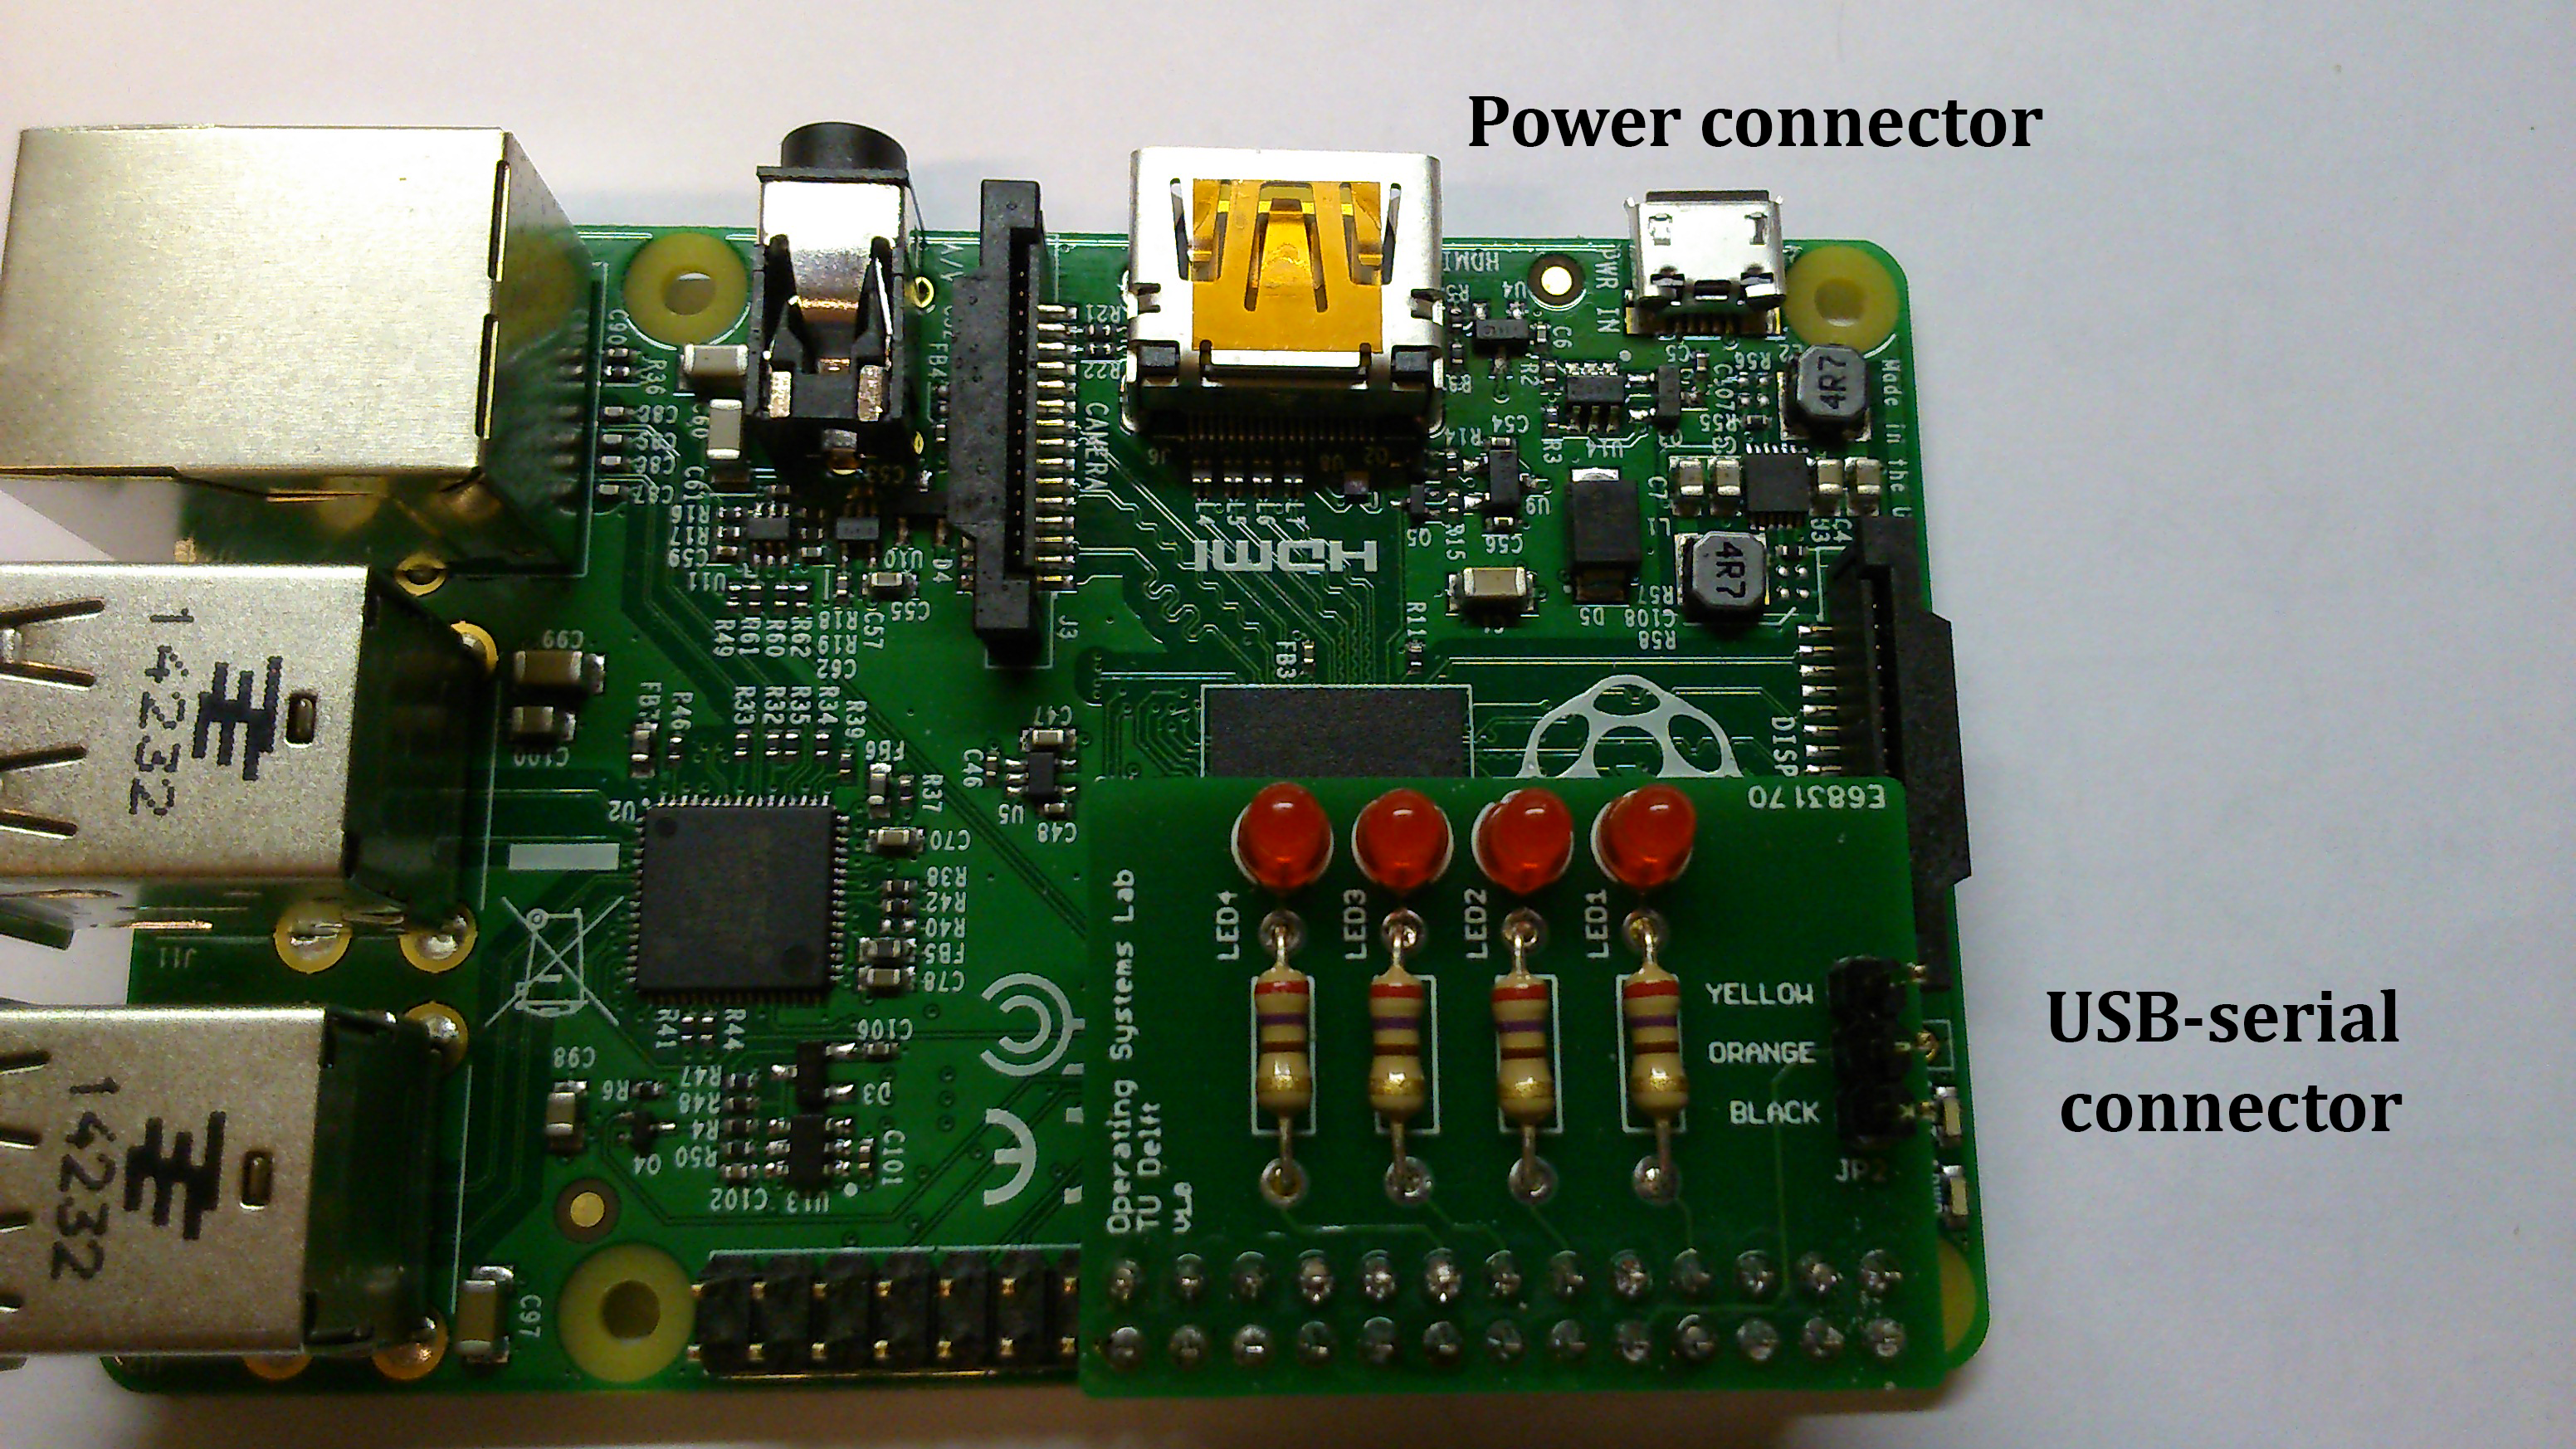
\includegraphics[width=0.80\textwidth]{images/setup.png}
	\caption{Raspberry Pi with extension board}
	\label{fig:raspberry-setup}
\end{figure}


\section{Programming Environment}
\label{sec:environment}
In order to successfully program the supplied hardware, you need an operating system with a compiler. Dozens operating systems exists, however to guarantee functionality and service we will only support the operating systems mentioned below. Please feel free to chose either of these operating systems.

\subsection*{Windows}
As mentioned before you will be using a serial cable as a connecting gateway between the computer and raspberry pi. In the case you are using your own windows powered laptop, it is necessary to install the corresponding drivers. In that case - if you have not already done so - install the PL2303 drivers. These can be downloaded from: \url{http://www.prolific.com.tw/US/ShowProduct.aspx?p_id=225&pcid=41}\\

Follow the steps mentioned on that page to install the driver. The driver is installed in such a way that when you later plug in the USB console lead, it will still launch the ``Found New Hardware'' wizard. If you allow the Wizard to search the Internet and install the drivers, it should work. When you have successfully installed the drivers you will be able to connect to your Raspberry Pi through the Console Lead.\\ 

Before you are able to connect to the device, you need to know to which communication port the Raspberry Pi is connected. You can find this by looking in the \menu{Ports} section of the \menu{Windows Device Manager} which is accessible through \menu{Control Panel} under \menu{System}.\\

The program you need to use for connecting with the Raspberry Pi is called Putty. You can download putty from the website \url{http://www.putty.org}. If you are using an x86 machine you can directly download putty via \url{http://goo.gl/BgbXpy}. It should be noted that Putty is not an installer but the actual program itself. Therefore, no installation is required to run Putty.\\
\begin{figure}[!htbp]
	\centering
		\includegraphics[width=0.80\textwidth]{images/putty-config.jpg}
	\caption{Example configuration for Putty}
	\label{fig:putty-config}
\end{figure}

When you open Putty you have to select the connection type \signal{Serial} from the radio buttons and set the speed to \signal{115200} and the serial line to the com port number you found in the previous paragraph. Additionally, please see figure \ref{fig:putty-config}. If the setup is correct you can open the connection and a console screen will be opened (see figure \ref{fig:console-windows}). Here you have to login with username \menu{pi} and password \menu{raspberry}.

\begin{figure}[!htbp]
	\centering
		\includegraphics[width=0.80\textwidth]{images/console-windows.jpg}
	\caption{Console screen on Windows PC}
	\label{fig:console-windows}
\end{figure}

\subsection*{Linux}
If you use Linux it is not needed to install additional software as the \signal{screen} package is included. However in some Linux distributions such as Ubuntu 12.10, the \signal{screen} package is not included. In this case you will have to install the package. You can do this by typing the following command.

\begin{flushleft}
	\code{sudo apt-get install screen}
\end{flushleft}

In order to find to which TTY port the Raspberry Pi is connected, execute the following command:

\begin{flushleft}
    \code{dmesg | grep tty}
\end{flushleft}

Now if you want to connect to the Raspberry Pi (in this case connected to /dev/ttyUSBO as found in the previous step) you type the following command.

\begin{flushleft}
	\code{screen /dev/ttyUSB0 115200}
\end{flushleft}

When your connection is successfully initialised you will see the screen of figure \ref{fig:console-linux}.

\begin{figure}[!htbp]
	\centering
		\includegraphics[width=0.80\textwidth]{images/console-linux.jpg}
	\caption{Console screen Linux}
	\label{fig:console-linux}
\end{figure}


		\part{Assignments}
			\chapter[Session 1: Introduction to C and Processes]{Introduction to C and Processes}\label{chap:session1}
\chaptermark{Introduction to C and Processes}
In previous classes you all have had classes that utilised C as a programming language. This first lab session is used to get to know the environment you will be working with as well as compiling the code you will be going to write.

The objectives of this session are listed below.
	\begin{itemize}
		\item Become familiar with the Raspberry Pi
		\item Write some simple C programs
		\item Learn how to compile a C program
		\item Learn what a process is and what it does
	\end{itemize}

\section{Assignments}
This first lab session consist of 3 assignments. In these assignments you have to write different programs which will be executed on the Raspberry Pi.

Early computers allowed only one program to be executed at a time. This program had complete control of the system and had access to all the system’s resources. In contrast, contemporary computer systems allow multiple programs to be loaded into memory and executed concurrently. The later case requires you to write a program, compile it and finally run it on a computer as a process. A process it a program that is in execution.Your program becomes a process of the Linux operating system. You could use the command \code{ps} in the console screen to list all the current processes of the system. 

\begin{info}
To make it easier to assess your assignments you have to write them in different files and you have to write enough comments in your code. We will assess you accordingly!
\end{info}

\subsection*{Assignment 1.1}
For the first assignment you have to write a small program. The file with the code of the program must uploaded to the Raspberry Pi followed by a compilation of your code to get the actual program. Once you have performed the compiling step, you could run the program. The program you have to write has some simple objectives which are listed below. Keep in mind that when this program runs on the Raspberry Pi it has become a process of the Linux Operating System.
	\begin{objectives}
		Objectives for a correct implementation of Assignment 1.1
		\begin{itemize}[noitemsep]
			\item Create variables with your name and student number
			\item Make sure your program is able to print your name and student number in an organised way!
			\item Print the ID of the process that runs your program!
		\end{itemize}
	\end{objectives}
Once your implementation complies with these objectives, you have to upload your solution to the Raspberry Pi and compile it with the GCC compiler of the Raspberry Pi. You could use a makefile for the compilation step which should make it easier to compile it again. When you run this program multiple times you will see that it gets a different process ID each time you run the program. Explain why this is the case.\\
\signature

\subsection*{Assignment 1.2}
In this assignment you have to write a program that is able to execute commands that you will usually use in your command window. The objective of this task is to become familiar with two different ways of executing Linux commands within a C program. For this assignment you have to write a program that creates a folder in the folder where your program is executed and you have to execute the function to list all the files and directories in the current folder. 
	\begin{objectives}
		Objectives for a correct implementation of Assignment 1.2
		\begin{itemize}[noitemsep]
			\item Create a folder
			\item List all files and directories in the current directory
			\item Use 2 different functions to realise the above objectives
		\end{itemize}
	\end{objectives}
	\signature

\subsection*{Assignment 1.3}
In the previous two assignments you wrote a program which was executed as a process on the Raspberry Pi. In assignment 1.3 you will extend assignment 1.2 with the functionality to run another process. This so called "child" process has to execute the same code as the main program. The objectives of this assignment are also listed below.
	\begin{objectives}
		Objectives for a correct implementation of Assignment 1.3
		\begin{itemize}[noitemsep]
			\item Create a "child" process which runs the same code as the main program
			\item Create a if/else statement to print which process is active (child or parent)
			\item The parent process has to wait for the child process before it is finished
		\end{itemize}
	\end{objectives}
	\signature

\section{Bonus Question: UNIX Shell and History Feature}
This project consists of designing a C program to serve as a shell interface that accepts user commands and then executes each command in a separate process. This project can be completed on any Linux, UNIX, or Mac OS X system.
A shell interface gives the user a prompt, after which the next command is entered. The example below illustrates the prompt osh> and the user’s next command: \code{cat prog.c}. (This command displays the file prog.c on the terminal using the UNIX cat command.)
\begin{flushleft}
    \code{osh> cat prog.c}
\end{flushleft}

One technique for implementing a shell interface is to have the parent process first read what the user enters on the command line (in this case, cat prog.c), and then create a separate child process that performs the command. Unless otherwise specified, the parent process waits for the child to exit before continuing. However, UNIX shells typically also allow the child process to run in the background, or concurrently. To accomplish this, we add an ampersand (\&) at the end of the command. Thus, if we rewrite the above command as

\begin{flushleft}
    \code{osh> cat prog.c \&}
\end{flushleft}

the parent and child processes will run concurrently.
The separate child process is created using the \code{fork()} system call, and the user's command is executed using one of the system calls in the \code{exec()} family.
A C program that provides the general operations of a command-line shell is supplied below. The \code{main()} function presents the prompt \code{osh->} and outlines the steps to be taken after input from the user has been read. The \code{main()} function continually loops as long as should run equals 1; when the user enters exit at the prompt, your program will set should run to 0 and terminate.
This project is organised into two parts: (1) creating the child process and executing the command in the child, and (2) modifying the shell to allow a history feature.
\begin{lstlisting}
#include <stdio.h>
#include <unistd.h>

#define MAX_LINE 80 /* The maximum length command */

int main(void) {
   char *args[MAX_LINE/2 +1]; /* command line arguments */
   int should_run = 1; /* flag to determine when to exit program */
   
   while (should_run) {
      printf("osh>");
      fflush(stdout);
      
      /**
       * After reading user input, the steps are:
       * (1) fork a child process using fork()
       * (2) the child process will invoke execvp()
       * (3) if command included &, parent will invoke wait()
       */
    }
    
    return 0;
}
\end{lstlisting}

\subsection*{Part 1: Creating a Child Process}
The first task is to modify the \code{main()} function as mentioned above so that a child process is forked and executes the command specified by the user. This will require parsing what the user has entered into separate tokens and storing the tokens in an array of character strings. For example, if the user enters the command \code{ps -ael} at the \code{osh>} prompt, the values stored in the args array are:
\begin{flushleft}
args[0] = ``ps''\\
args[1] = ``-ael''\\
args[2] = NULL
\end{flushleft}

This args array will be passed to the \code{execvp()} function, which has the following prototype:
\begin{flushleft}
\code{execvp(char *command, char *params[]);}
\end{flushleft}

Here, command represents the command to be performed and params stores the parameters to this command. For this project, the \code{execvp()} function should be invoked as \code{execvp(args[0], args)}. Be sure to check whether the user included an \& to determine whether or not the parent process is to wait for the child to exit.

\subsection*{Part 2: Creating a History Feature}
The next task is to modify the shell interface program so that it provides a history feature that allows the user to access the most recently entered commands. The user will be able to access up to 10 commands by using the feature. The commands will be consecutively numbered starting at 1, and the numbering will continue past 10. For example, if the user has entered 35 commands, the 10 most recent commands will be numbered 26 to 35.
The user will be able to list the command history by entering the command
\begin{flushleft}
\code{history}
\end{flushleft}
at the \code{osh>} prompt. As an example, assume that the history consists of the commands (from most to least recent):
\begin{flushleft}
\code{ps, ls -l, top, cal, who, date} 
\end{flushleft}
The command history will output:\\
\code{
     6 ps\\
     5 ls -l\\
     4 top\\
     3 cal\\
     2 who\\
     1 date\\
     }
Your program should support two techniques for retrieving commands from the command history:
\begin{objectives}
\begin{itemize}[noitemsep]
\item When the user enters !!, the most recent command in the history is executed.
\item When the user enters a single ! followed by an integer N, the Nth command in the history is executed.
\end{itemize}

Continuing our example from above, if the user enters !!, the ps command will be performed; if the user enters !3, the command cal will be executed. Any command executed in this fashion should be echoed on the user’s screen. The command should also be placed in the history buffer as the next command.
The program should also manage basic error handling. If there are no commands in the history, entering !! should result in a message ``No commands in history.'' If there is no command corresponding to the number entered with the single !, the program should output ``No such command in history.''
\end{objectives}
\signature

			\chapter[Session 2: Thread]{Threads}\label{chap:session2}
\chaptermark{Threads}
The second session of this lab will contain some exercises about threads. In session \ref{chap:session1} you learned about process and how they work. In this assignment you will use threads and these threads will be used in all other session of this lab. The objectives of this session are listed below.
	\begin{itemize}
		\item Learn what a thread is and how you could create one
		\item Learn how you could use the I/O interface of the Raspberry Pi
	\end{itemize}

\section{Assignments}
In the previous assignment you already learned something about processes on a Linux system. In this second assignment you will learn something about threads. 

A thread is a basic unit of CPU utilisation; it comprises a thread ID, a program counter, a register set, and a stack. It shares with other threads belonging to the same process its code section, data section, and other operating-system resources, such as open files and signals. A traditional (or heavyweight) process has a single thread of control. If a process has multiple threads of control, it can perform more than one task at a time. Since each unique thread has its own memory, it is a lot faster to create and destroy threads. 

\begin{figure}
  \centering
  \includegraphics[width=.8\textwidth]{images/thread.pdf}
\caption{Single-Threaded and Multi-Threaded Processes}
\label{fig:thread}
\end{figure}

In this session you will learn how to create threads. The concept of threads will be further utilised by all the other assignments of this lab. The next session is about multithreading and the advantage of threads above processes.

\subsection*{Using I/O on Raspberry Pi}\label{sec:io-intro}
This tutorial will state information with regards to the input/output (I/O) functionalities of the Raspberry Pi. To make it easy, we will use a library which provides a set of functions to communicate with the I/O pins of the Raspberry Pi. This lab will use the Wiring Pi library. This tutorial will mention the basic functions you have to use during this lab. If you want to use more advanced functions you could find a detailed reference on the website of WiringPi \url{http://www.wiringpi.com/reference}

Before using the WiringPi I/O library, you need to include its header file in your programs:

\begin{lstlisting}
#include <wiringPi.h>
\end{lstlisting}
Due to the fact that you will be using a non-standard library, do not forget to link the library when compiling your file. Therefore you could use the following line:

	\begin{codeblock}
		-I/usr/local/include -L/usr/local/lib -lwiringPi
	\end{codeblock}
When you have successfully included the library you are able use the WiringPi functions. The first thing you have to do is to call the function \code{wiringPiSetup()}:

\begin{lstlisting}
// Setup WiringPi
wiringPiSetup();
\end{lstlisting}
Once you have called the function \code{wiringPiSetup()} you are able to set the mode of the pins. Each pin can be set to several modes and therefor you have to select the right one in order to operate the pin correctly. To select the different pin modes you could use the function \code{pinMode(int pin, int mode);}:

\begin{lstlisting}
// Set LED1 pin to output
pinMode(LED1, OUTPUT);
\end{lstlisting}

Another function you will be going to use is the function to change the output value of the LED pins in order to turn the LED on or off. You could change the output value low or high by the function \code{digitalWrite (int pin, int value);}

\begin{lstlisting}
// Turn LED on
digitalWrite(LED1, HIGH);

// Turn LED off
digitalWrite(LED1, LOW);
\end{lstlisting}

The previously stated functions will allow you to turn the LED's on or off, more specifically the first function turns LED1 on, and the second one turns it off. The functions mentioned below can be used to control the LED's with a Pulse Width Modulated signal (PWM). PWM can be used to control the brightness of the LED's. Additionally PWM can be used to fade-in and fade-out the LED's. The LED's which you will be going to control with PWM signals must be initialised different than just turning LED's on and off. The function \code{softPwmCreate (int pin, int initialValue, int pwmRange);} is used to initialise the LED. In this function you have to enter a initial value (0 for off and 100 for fully  on) and the pwmRange which should be 100. 

The function \code{softPwmWrite(int pin, int value);} is used to update the PWM value of the LED. We use for PWM the soft PWM library because there is only one pin on the Raspberry Pi which allows hardware PWM. Soft PWM means a thread is created which controls the LED to the corresponding PWM value. Before you can use the functions for PWM you have to include the soft PWM library. \code{\#include <softPwm.h>}

\begin{lstlisting}
// Include headers
#include <wiringPi.h>
#include <softPwm.h>

// Initialise pin for PWM output
softPwmCreate(LED1, 0, 100);

// Update the PWM value of a LED
softPwmWrite(LED1, 50);
\end{lstlisting}

\subsection*{Assignment 2.1}
The objective of this assignment is creating a new thread. You have to include the POSIX Thread library in order to create a thread in your main function. The only thing you have to implement in your main function is the creation of a thread, waiting for the thread to finish and killing the program. The complete list of objectives of this assignment are listed below.
	\begin{objectives}
		Objectives for a correct implementation of Assignment 2.1
		
		The main function must create a thread, wait till the thread is finished and finally close the program. The objectives of the thread are listed below.
		\begin{itemize}
			\item Print the thread ID and function name of the thread
			\item Create a counter which counts from 1 to 10 and wait 1 second between each increment
		\end{itemize}
	\end{objectives}
	\signature

\subsection*{Assignment 2.2}
In this assignment you will - just as in assignment 2.1 - create a thread. Basically the same main functions can be used. However, instead of using a timer you will use the input/output port of the Raspberry Pi. In this assignment you have to use the output function of this port to blink multiple LED's. The objectives of this assignment are listed in the grey box below.
	\begin{objectives}
		Objectives for a correct implementation of Assignment 2.2
		
		The main function must create a thread, wait till the thread is finished and finally close the program. The objectives of the thread are listed below.
		\begin{itemize}
			\item Initialise the LED pins as output
			\item Create a certain pattern with the LED's
			\item Close the thread after 20 seconds
		\end{itemize}
		
		The pattern named above may be every pattern you want. It could be some difficult pattern or just simple blinking of LED's
	\end{objectives}
	\signature
	
\section{Bonus Question: Sudoku Solution Validator}
\label{sec:sudoku}
A Sudoku puzzle uses a 9 × 9 grid in which each column and row, as well as each of the nine 3 × 3 subgrids, must contain all of the digits 1···9. Figure \ref{fig:sudoku} presents an example of a valid Sudoku puzzle. This project consists of designing a multithreaded application that determines whether the solution to a Sudoku puzzle is valid.
There are several different ways of multithreading this application. One suggested strategy is to create threads that check the following criteria:
\begin{itemize}
\item A thread to check that each column contains the digits 1 through 9
\item A thread to check that each row contains the digits 1 through 9
\item Nine threads to check that each of the 3 × 3 subgrids contains the digits 1 through 9
\end{itemize}

\begin{figure}[hbp]
\centering
\includegraphics[width=0.5\textwidth]{images/sudoku.pdf}
\caption{Solution to a 9 x 9 Sudoku puzzle}
\label{fig:sudoku}
\end{figure}

This would result in a total of eleven separate threads for validating a Sudoku puzzle. However, you are welcome to create even more threads for this project. For example, rather than creating one thread that checks all nine columns, you could create nine separate threads and have each of them check one column.

\subsection*{Passing Parameters to Each Thread}
The parent thread will create the worker threads, passing each worker the location that it must check in the Sudoku grid. This step will require passing several parameters to each thread. The easiest approach is to create a data structure using a struct. For example, a structure to pass the row and column where a thread must begin validating would appear as follows:
\begin{lstlisting}
/* structure for passing data to threads */ 
typedef struct {
   int row;
   int column; 
} parameters;
\end{lstlisting}

Both Pthreads and Windows programs will create worker threads using a strategy similar to that shown below:
\begin{lstlisting}
parameters *data = (parameters *) malloc(sizeof(parameters)); 
data->row = 1;
data->column = 1;
/* Now create the thread passing it data as a parameter */
\end{lstlisting}

The data pointer will be passed to the \code{pthread create()} (Pthreads) function, which in turn will pass it as a parameter to the function that is to run as a separate thread.

\subsection*{Returning Results to the Parent Thread}
Each worker thread is assigned the task of determining the validity of a particular region of the Sudoku puzzle. Once a worker has performed this check, it must pass its results back to the parent. One good way to handle this is to create an array of integer values that is visible to each thread. The ith index in this array corresponds to the ith worker thread. If a worker sets its corresponding value to 1, it is indicating that its region of the Sudoku puzzle is valid. A value of 0 would indicate otherwise. When all worker threads have completed, the parent thread checks each entry in the result array to determine if the Sudoku puzzle is valid.\\
\signature


			\chapter[Session 3: Multithreading]{Multithreading}\label{chap:session3}
\chaptermark{Multithreading}
This lab session will dive into multithreading. In the previous assignments you learned the basics with regards to threads on a Linux system. In this assignment you will create a program that contains multiple threads. The objectives of this session are listed below:
	\begin{itemize}
		\item Learn the concept of multithreading
		\item Get to know the advantages and disadvantages of multitasking
	\end{itemize}

\section{Assignments}
A multithreaded process contains several different flows of control within the same address space. The benefits of multithreading include increased responsiveness to the user, resource sharing within the process, economy, and scalability factors, such as more efficient use of multiple processing cores. In the following assignments you have to write a program that consist of multiple threads. From these assignments it should become clear that threads are more easily to use than the regular processes. 

\subsection*{Assignment 3.1}
In the previous session you have learned how to create a single process. Processes can come in extremly handy but they suffer from a single point of failure. In this assignment you will get to know processes in a more advanced way, hoping to eludicate the advantages and disadvantages of multithreading processeses. You will use the LED extention board to visualy see what is going on. The objectives of this assignment are listed in the grey box below.
	\begin{objectives}
	    Objectives for a correct implementation of Assignment 3.1
	    
		Create a program (main function) that creates 3 threads. The program is only aloud to finish after the execution of all 3 threads! Lastly, you have to alter the output such that it outputs the currently active thread, it should correspond to the following structure: \code{[Thread?]:}. 
		
		\textbf{Thread 1 must implement:}
		\begin{itemize}[noitemsep]
			\item Blink the LED's with a certain self choosen pattern. This pattern could be whatever you want\\
		\end{itemize}
		
		\textbf{Thread 2 must implement:}
		\begin{itemize}[noitemsep]
			\item Count from 1 to 20 with 1 second in between each increment and print the updated counter value\\
		\end{itemize}
		
		\textbf{Thread 3 must implement:}
		\begin{itemize}[noitemsep]
			\item Create a 10x10 array with random numbers between 0 and 100 and print this array\\
		\end{itemize}
	\end{objectives}
	\signature 

\subsection*{Assignment 3.2}
In the previous assignment you created three processes that operated in a multithreaded regime. This assignment has the same method of approach. The difference lies in the difficulty of the assignment as this assignment will introduce binary counting! The objectives of this assignment are listed below.
    \begin{objectives}
    Objectives for a correct implementation of Assignment 3.2
    
        Use the source code of the previous assignment and alter it such that the output meets the following requirements. Keep in mind that you still have to output to currently active thread according to the same convention as mentioned in assignment 3.1
        
        \textbf{Thread 1 must implement:}
        \begin{itemize}
        \item Use the LED's on the extention board to make a binary counter which binary counts from zero to 10 and back to zero with 1 second in between each incremation. So for the value $5_{dec}$ the binary value is $0101_{bin}$ outputed and only LED's 1 and 3 should be active!
        \end{itemize}
        
        \textbf{Thread 2 must implement:}
        \begin{itemize}
        \item Make a counter from 10 to 0 and back to 10.
        \end{itemize}
        
        \textbf{Thread 3 must implement:}
        \begin{itemize}
        \item Rearrange the array created in the previous assignment in such a way the first column has ascending numbers\\
        \end{itemize}
    \end{objectives}
\signature
    
\subsection*{Assignment 3.3}
Write a multithreaded program that calculates various statistical values for a list of numbers. This program will be passed a series of numbers on the command line and will then create three separate worker threads. One thread will determine the average of the numbers, the second will determine the maximum value, and the third will determine the minimum value. For example, suppose your program is passed the integers:
\begin{flushleft}
	\code{90 81 78 95 79 72 85}
\end{flushleft}
 The program will report:
The average value is 82
The minimum value is 72 
The maximum value is 95

The objectives of this assignment are listed below
\begin{objectives}
Objectives for a correct implementation of Assignment 3.3

\begin{itemize}
\item The program must be able to listen to input values (sanitize the input to check if it is valid!)
\item Compute the average value
\item Compute the minimum value
\item Compute the maximum value
\item Compute the median value
\item Compute the standard deviation
\item Determine how many threads you should be using to assure a fast execution of the program.
\end{itemize}
\end{objectives}
\signature

\section{Bonus Question: Multithreaded Sorting Application}
Write a multithreaded sorting program that works as follows: A list of integers is divided into two smaller lists of equal size. Two separate threads (which we will term \textbf{sorting threads}) sort each sublist using a sorting algorithm of your choice. The two sublists are then merged by a third thread — a \textbf{merging thread} — which merges the two sublists into a single sorted list.

\begin{figure}[hbp]
\centering
\includegraphics[width=0.5\textwidth]{images/multisort.pdf}
\caption{Multithreaded Sorting}
\label{fig:multi}
\end{figure}

Because global data are shared cross all threads, perhaps the easiest way to set up the data is to create a global array. Each sorting thread will work on one half of this array. A second global array of the same size as the unsorted integer array will also be established. The merging thread will then merge the two sublists into this second array. Graphically, this program is structured according to Figure \ref{multi}.
This programming project will require passing parameters to each of the sorting threads. In particular, it will be necessary to identify the starting index from which each thread is to begin sorting. Refer to the instructions of section \ref{sec:sudoku} for details on passing parameters to a thread. The parent thread will output the sorted array once all sorting threads have exited.\\
\signature


			\chapter[Session 4: Scheduling of threads]{Scheduling of threads}\label{chap:session4}
\chaptermark{Scheduling of threads}
In the previous sessions you have learnt what a thread is, how to create one and how to create multiple threads. But can the total running time of this execution be optimised? This chapter is going to introduce scheduling as a possible optimisation. The objectives of this session are listed below.\\

\begin{itemize}
\item To introduce CPU scheduling, which is the basis for multiprogrammed operating systems.
\item To understand the difference between process scheduling and thread scheduling.
\end{itemize}

\newpage
\section{Assignments}
\begin{wrapfigure}{r}{0.5\textwidth}
  \vspace{-20pt}
  \begin{center}
    \includegraphics[width=0.48\textwidth]{images/schedule.pdf}
  \end{center}
  \vspace{-20pt}
  \caption{Alteration of IO and CPU bursts}
\end{wrapfigure}
In a single-processor system, only one process can run at a time. Others must wait until the CPU is free and can be rescheduled. The objective of multiprogramming is to have some process running at all times, to maximise CPU utilisation. The idea is relatively simple. A process is executed until it must wait, typically for the completion of some I/O request. In a simple computer system, the CPU then just sits idle. All this waiting time is wasted; no useful work is accomplished. With multiprogramming, we try to use this time productively.\\
\vspace{20pt}
Several scheduling algorithms exists. CPU scheduling deals with the problem of deciding which of the processes in the ready queue is to be allocated the CPU. You can find some scheduling algorithms below.
\begin{itemize}
\item First-Come, First-Served Scheduling (FCFS)
\item Shortest-Job-First Scheduling (SJF)
\item Priority Scheduling
\item Round-Robin Scheduling (RR)
\item Multilevel Queue Scheduling
\item Multilevel Feedback Queue Scheduling
\end{itemize}

\newpage
\subsection*{Assignment 4.1}
In order to schedule processes fairly, a round-robin scheduler generally employs time-sharing, giving each job a time slot or quantum (its allowance of CPU time), and interrupting the job if it is not completed by then. The job is resumed next time a time slot is assigned to that process. In the absence of time-sharing, or if the quanta were large relative to the sizes of the jobs, a process that produced large jobs would be favoured over other processes. Round Robin algorithm is a pre-emptive algorithm as the scheduler forces the process out of the CPU once the time quota expires. You will use Round-Robin as a scheduling algorithm in this assignment.\\ 

Use your your solution to assignment 3.2 and change the scheduling method. The threads must have different priorities and use Round-Robin as the desired scheduling method. Implement this assignment such that you can show that the priorities are changed and have indeed influenced the way of executing the code.

\begin{objectives}
Objectives for a correct implementation of Assignment 4.1


\begin{itemize}
\item Implement Round-Robin as scheduling algorithm.
\item Prove that priorities change when implementing RR.
\end{itemize}
\end{objectives}
\signature

\subsection*{Assignment 4.2}
By far the simplest CPU-scheduling algorithm is the first-come, first-served (FCFS) scheduling algorithm. With this scheme, the process that requests the CPU first is allocated the CPU first. The implementation of the FCFS policy is easily managed with a FIFO queue. This assignment has the same objectives as assignment 4.1. The only difference is that you will be utilising the FCFS scheduling algorithm as apposed to the Round-Robin scheduling algorithm.
\begin{objectives}
Objectives for a correct implementation of Assignment 4.2

\begin{itemize}
\item Implement FCFS as scheduling algorithm.
\item Beeing able to explain in detail the difference between FCFS and other scheduling algorithms!
\end{itemize}
\end{objectives}
\signature

\section{Bonus Questions}
Below you will find three questions. If you answer all these questions correctly, you will be rewarded a bonus!\\

\subsection*{Question 1}
Which of the following scheduling algorithms could result in starvation?
You will have to explain to the assistants which one(s) could result in starvation so be prepared!

\begin{itemize}
\item first-come, first-served
\item Shortest job first
\item Round Robin
\item Priority
\end{itemize}
\signature 

\subsection*{Question 2}
Consider a variant of the RR scheduling algorithm in which the entries in the ready queue are pointers to the PCBs.

\begin{itemize}
\item What would be the effect of putting two pointers to the same process in the ready queue?
\item What would be two major advantages and two disadvantages of this scheme?
\item How would you modify the basic RR algorithm to achieve the same effect without the duplicate pointers?
\end{itemize}
\signature

\subsection*{Question 3}
Consider the scheduling algorithm in the Solaris operating system for time-sharing threads.
\begin{itemize}
\item What is the time quantum (in milliseconds) for a thread with priority 15? With priority 40?
\item Assume that a thread with priority 50 has used its entire time quantum without blocking. What new priority will the scheduler assign this thread?
\item Assume that a thread with priority 20 blocks for I/O before its time quantum has expired. What new priority will the scheduler assign this thread?
\end{itemize}

\signature

			\input{Part2/session5}

		\appendix
	
	
	% X. van Rijnsoever, 2014
\cleartoevenpage
\thispagestyle{empty}
\AddToShipoutPicture*{
	\setlength{\unitlength}{1cm}
	\put( 0,  0){\includegraphics{images/TUDelft_border_back}}
}
~


\end{document}
